\documentclass{article} 
\usepackage{nips14submit_e,times}
\usepackage{hyperref}
\usepackage{url}
\usepackage{graphicx}
\usepackage{footmisc}
\usepackage{amsmath}
\usepackage{subcaption}

\title{Network Dynamics in Citation Graphs}

\author{
    Puneeth Vishisth R\thanks{For Python code, data, and all figures, please visit my git repository- \url{https://github.com/HULK050707/HSN619_Project_21322024}} \\
    Humanities and Social Sciences \\
    Indian Institute of Technology Roorkee \\
    Roorkee - 247667 \\
    \texttt{puneeth\_vr@hs.iitr.ac.in}
}

\newcommand{\fix}{\marginpar{FIX}}
\newcommand{\new}{\marginpar{NEW}}

\nipsfinalcopy % Uncomment for camera-ready version

\begin{document}

\maketitle

\begin{abstract}
In this paper, I mainly focus on citation networks, which are directed social networks where nodes represent academic papers and edges represent citations. These networks provide a representation of a paper's influence and academic strength within the academic community. Basic network concepts are applied in this report to study the structure of citation networks, develop a model based on cascading concepts, perform a temporal analysis to identify trends, and examine possible effects of citation aging.
\end{abstract}

\section{Introduction}
\label{headings}
Citation networks are social networks where nodes represent academic papers and edges represent citations made between these papers. These networks provide some insight into the academic influence of papers, as the number of citations (the degree of a node) often indicates the strength and impact of a paper within the academic community. Metrics such as the H-index, commonly used to measure academic impact, are also grounded in principles of network theory, highlighting the importance of citation networks in understanding academic influence.

The initial focus was to replicate a study based on citation networks and using similar data. The study aimed to predict centrality using AI/ML models. However, as I started to explore the data, I shifted towards a more fundamental approach, aiming to practically apply basic network theory concepts learned during the course. From degree distribution and centrality to building a model on cascading effects, I analyze the results using these real-world citation networks. I also try to perform a temporal analysis on this network to observe how the network evolves and the changes in the importance of nodes as the network grows.

\section{Literature Review}
\label{headings}
Initially, I tried to replicate a course project by Mark Holmstrom [1], but as I started working with the data, I found it fascinating to apply the concepts of network theory from the course and Barabási's network science book [2]. For the coding and implementation, I relied on the NetworkX library [3], using its documentation and example graphs to plot and analyze the network structures.

I also reviewed the paper "Citation Networks in High-Energy Physics" by Lehmann, Lautrup, and Jackson [4], which studies the structural patterns formed by citation networks. This study highlights the formation of hierarchical and scale-free networks in high-energy physics.

\section{Network Analysis}
\label{headings}
In this project, I conduct four key analyses using empirical data to explore the structure and dynamics of citation networks. First, I examine the degree distribution to determine if it aligns with the characteristics of scale-free networks, a real-world network property. I then investigate centrality measures to identify influential nodes and observe the network's structure through visualizations, summary metrics, and plots. Following this, I develop a model based on cascading effects to study how node influence propagates within the network, focusing on the role of key nodes in the theoretical physics community.

Finally, I perform a temporal analysis to track changes over time, examining shifts in the degree of specific nodes and the average degree across the network. This helps to visualize trends, such as citation aging and evolving patterns of academic influence in the theoretical physics community. 

\subsection{Dataset and Network Formation}
\begin{figure}[h]
\centering
\begin{subfigure}[b]{0.40\textwidth}
    \centering
    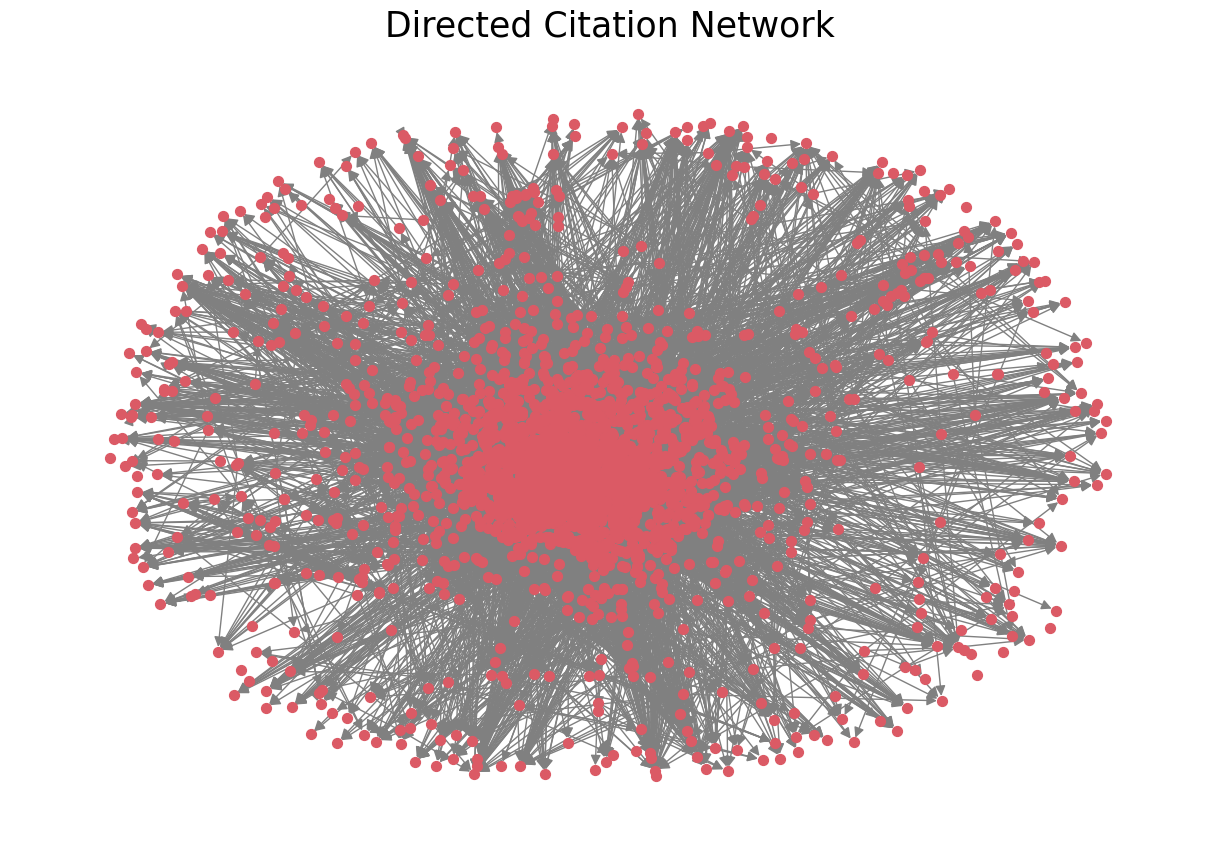
\includegraphics[width=\textwidth]{Figures/Network Graph.png}
    \caption{Complete citation network}
    \label{fig:network_graph}
\end{subfigure}
\hfill
\begin{subfigure}[b]{0.40\textwidth}
    \centering
    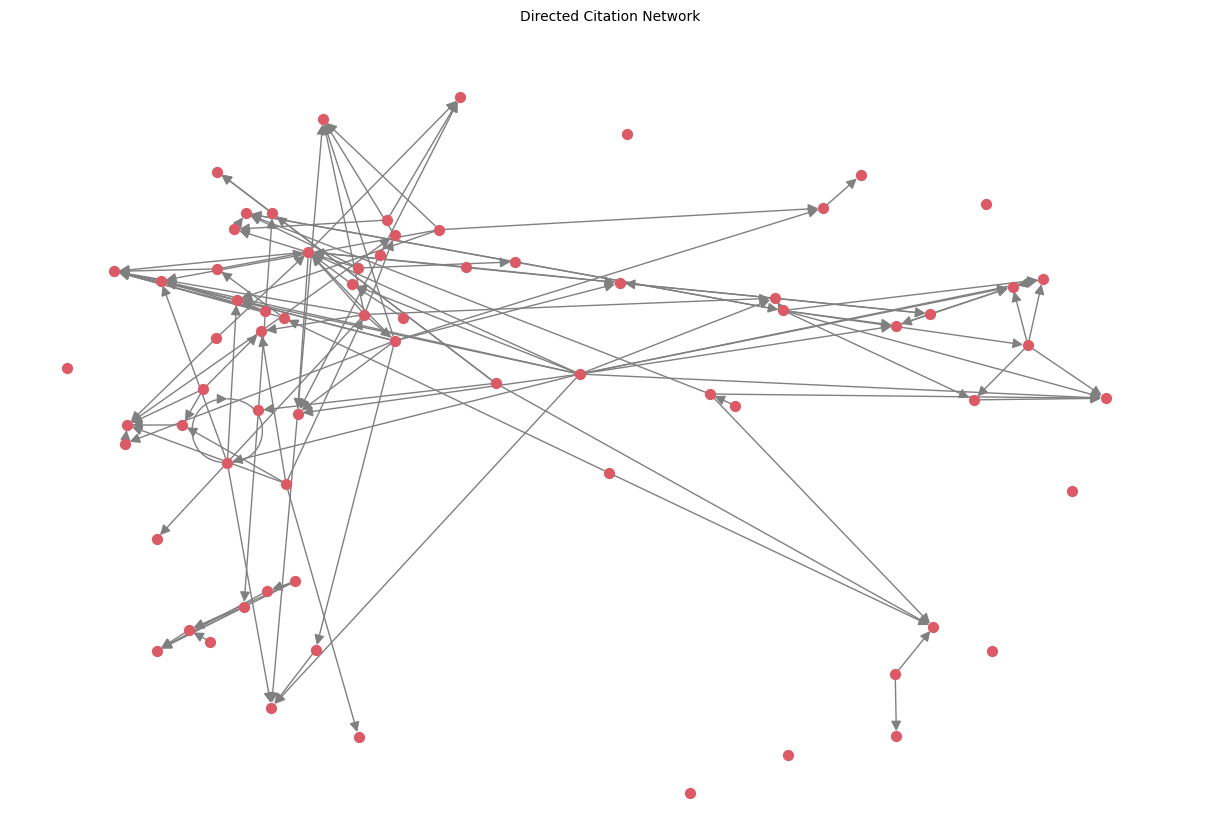
\includegraphics[width=\textwidth]{Figures/sample network.png}
    \caption{Sample nodes from the network}
    \label{fig:sample_network}
\end{subfigure}
\caption{Graphed directed citation network, sample network figure is for better visualisation}
\label{fig:combined}
\end{figure}

For this analysis, I used publicly available data from the SNAP website [5]
\footnote{http://snap.stanford.edu/data/cit- HepTh.html} 
specifically the Arxiv HEP-TH (High Energy Physics Theory) citation graph
\footnote{The data covers papers in the period from 1993 to 2003 (124 months). It begins within a few months of the inception of the arXiv, and represents essentially the complete history of its HEP-TH section.}
This dataset includes citations from the e-print arXiv and covers 27,770 papers with 352,807 directed edges. Each edge represents a citation, where a directed edge from paper i to paper j indicates that paper i cites paper j. However, if a paper cites or is cited by a paper outside the dataset, that information is not included. The dataset also provides publication dates and meta-information on each paper.

\begin{table}[h]
    \centering
    \begin{tabular}{ll}
        \hline
        \textbf{Dataset statistics} & \\
        \hline
        Nodes & 27,770 \\
        Edges & 352,807 \\
        Nodes in largest WCC & 27,400 (0.987) \\
        Edges in largest WCC & 352,542 (0.999) \\
        Nodes in largest SCC & 7,464 (0.269) \\
        Edges in largest SCC & 116,268 (0.330) \\
        Average clustering coefficient & 0.3120 \\
        Number of triangles & 1,478,735 \\
        Fraction of closed triangles & 0.04331 \\
        Diameter (longest shortest path) & 13 \\
        90-percentile effective diameter & 5.3 \\
        \hline
    \end{tabular}
    \caption{Statistics of the dataset}
    \label{tab:dataset_stats}
\end{table}

I have selected this data because it is manageable in size and includes temporal data, which is crucial for observing how the network evolves over time. The meta-information on individual papers allows for further investigation into significant nodes.

I used a sample of nodes to create the network figure, as visualizing the entire network with 27,770 nodes is challenging. However, I also graphed the complete network, shown in Figure 1, which reveals a clear pattern with nodes densely concentrated in the central region. A separate graph with a subset of randomly sampled nodes is provided to better visualize the citation directions and improve understanding of the network structure.

\subsubsection{Degree Distribution}
In this section, I begin by plotting the degree distribution to analyze the type of network, i.e., whether it is random or scale-free, and attempt to fit a suitable function to the data. 

\begin{figure}[h]
\begin{center}
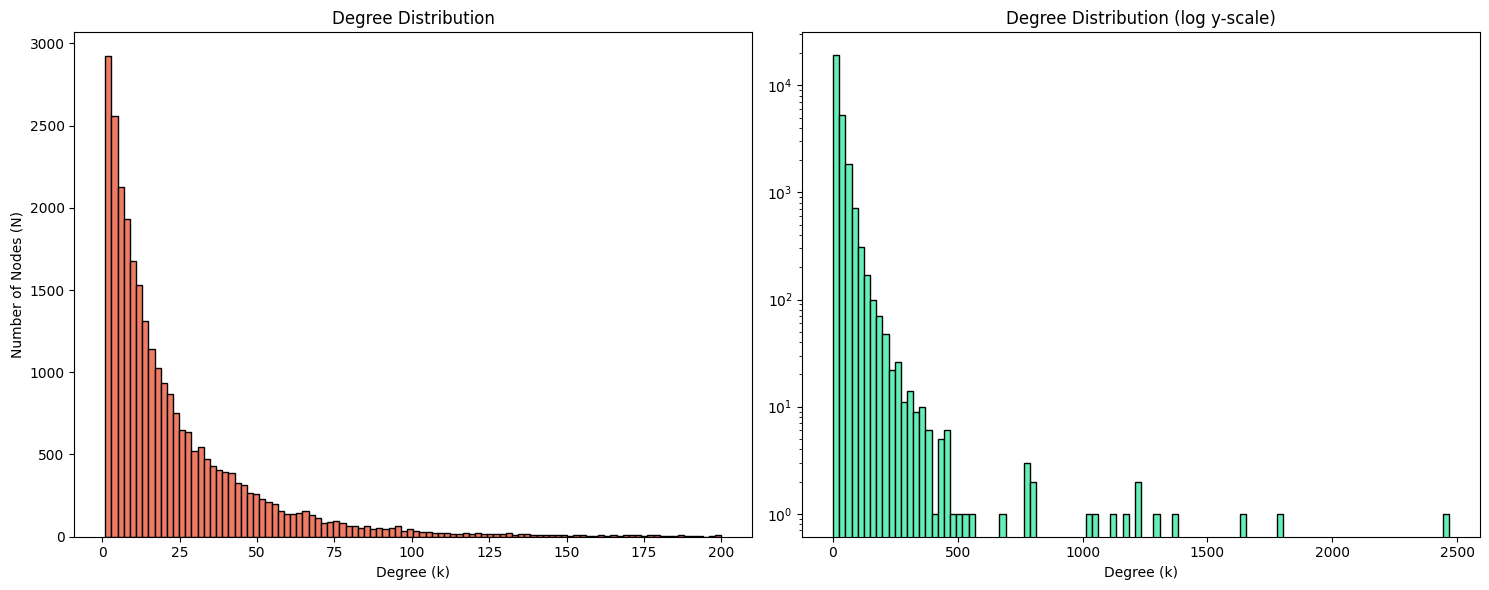
\includegraphics[width=1\textwidth]{Figures/Degree Distribution.png}
\end{center}
\caption{A plot of the degree (k) versus the number of nodes (n), showing the distribution of node degrees and the same distribution, but with a logarithmic scale applied to the y-axis}
\end{figure}

The plots of the Figure 2 clearly show that there are large number of nodes with small degree and low nodes having large degree. This implies that the citation network follow scale-free property. To confirm the property, we try fitting a best power law function using already existing libraries, which use regression models.

\begin{equation}
    P(k) = C \cdot k^{-\alpha}
    \label{eq:power_law}
\end{equation}

\begin{table}[h]
    \centering
    \begin{tabular}{ll}
        \hline
        Parameter & Value \\
        \hline
        Alpha ($\alpha$) & 3.1760678575019097 \\
        X min ($x_{\text{min}}$) & 62.0 \\
        R & 356.5777046915072 \\
        p & 2.771460206197671e-08 \\
        \hline
    \end{tabular}
    \caption{Calculating best minimal value for power law fit.}
    \label{tab:power_law_fit}
\end{table}

\begin{figure}[h]
    \centering
    \includegraphics[width=\textwidth]{Figures/Power Law Fit.png}
    \caption{Cummulative degree distribution to check nodes falling under Xmin}
    \label{fig:network_graph}
\end{figure}

1. Alpha ($\alpha$)$\>>$3 , implies a less skewed distribution, resembling random networks.\\
2. X min ($x_{\text{min}}$) = 62, is the threshold value of degree from which the power law behavior is observed.\\
3. A high positive R suggests that the power-law distribution provides a significantly better fit to the data compared to the alternative distribution.\\
4.A low p-value ($p < 0.05$) suggests that the null hypothesis (data follow a power-law distribution) can be rejected. Despite the high $R$, the power-law model may not perfectly explain the data.\\\\\\\\\

\begin{table}[h]
    \centering
    \begin{tabular}{lr}
        \hline
        \textbf{Metric} & \textbf{Value} \\
        \hline
        Total Nodes & 27,770 \\
        Nodes with degree $<$ X min & 26,655 \\
        Fraction of nodes with degree $<$ X min & 0.9598 \\
        \hline
    \end{tabular}
    \caption{Node Degree under X min}
    \label{tab:node_degree_info}
\end{table}

As observed in the Figure 3, Table 3 and Figure 4(a) we can see the power law fits better after degree 100, an fraction of nodes below X min(k=62) is high. This questions the power law property of the citation network.

\subsubsection{Degree Correlation}
Degree correlation quantifies the relationship between the degree of a node and the degrees of its neighboring nodes in a network. In the context of a citation network, degree correlation reveals how influential papers (nodes with high degrees) are connected to other influential or less influential papers, impacting the flow of information and knowledge diffusion.

The degree correlation is often represented as the correlation between the node's degree ($k$) and the average degree of its neighbors ($\bar{k}$).

\[\text{Degree of node } n = k, \quad \text{Degree of its } i\text{th neighbor } = k_i\]

The mean degree of the adjacent nodes of $n$ is given by:
\begin{equation}
    \bar{k} = \frac{\sum_{i=1}^k k_i}{k}
    \label{eq:average_k}
\end{equation}

Figure 4(b) below gives the visual representation of the degree correlation existing in the network. The correlation coefficient between a node’s degree and the average degree of its neighbors is then calculated using Pearson’s correlation formula.

\begin{figure}[h]
\centering
\begin{subfigure}[b]{0.40\textwidth}
    \centering
    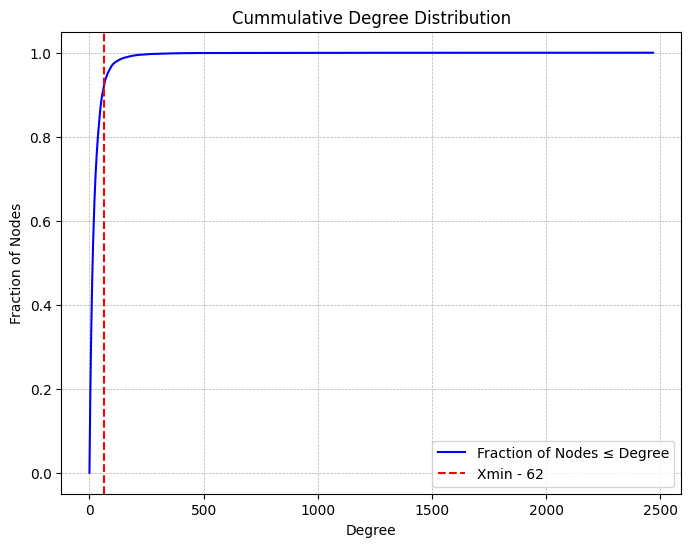
\includegraphics[width=\textwidth]{Figures/Cummulative Degree Distribution.png}
    \caption{Complete citation network}
    \label{fig:network_graph}
\end{subfigure}
\hfill
\begin{subfigure}[b]{0.40\textwidth}
    \centering
    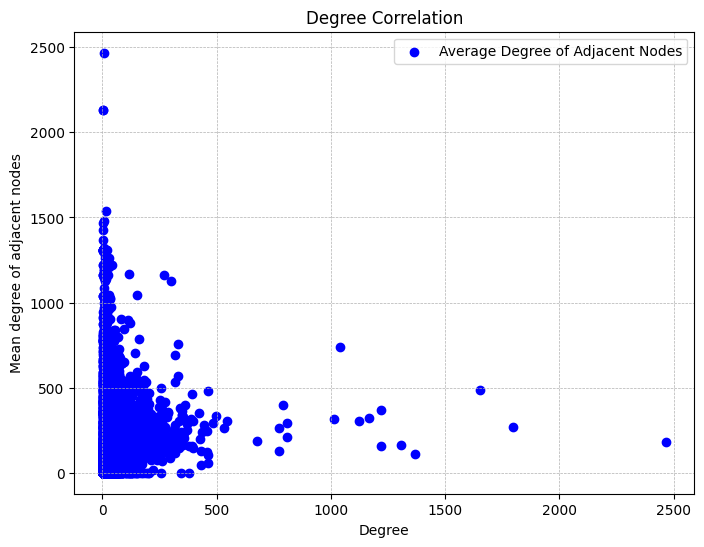
\includegraphics[width=\textwidth]{Figures/Degree Correlation}
    \caption{Degree Correlation}
    \label{fig:sample_network}
\end{subfigure}
\caption{Cummulative Degree Distribution with Xmin And Degree Correlation }
\label{fig:combined}
\end{figure}

\textbf{Result:} Correlation Coefficient = 0.2475

A positive coefficient (0.2475) indicates a mild assortative mixing in the network. This indicates that the nodes with a higher degree (highly cited papers) tend to connect more often to other nodes with higher degrees. However, the moderate coefficient highlights the complex nature of citations, where connections are influenced not only by paper strength but also by research areas, authorship, and collaborations.

\subsection{Centrality}
Centrality is a measure used in network analysis to determine the importance or influence of a node within a graph. It identifies nodes that play critical roles in connecting parts of the network, facilitating the flow of information, or holding high value[academic strength of node]. Common centrality metrics include betweenness centrality, in-degree centrality, closeness centrality, and eigenvector centrality. In this report I am mainly concerned with betweenness and in-degreee centrality.

\subsubsection{Betweenness Centrality}
In citation networks, betweenness centrality identifies nodes (papers/authors) that act as intermediaries connecting different parts of the network. For example, a paper linking two separate clusters, such as theoretical economics and mathematics, would have high betweenness centrality. Such a paper plays a crucial role in facilitating the transfer of knowledge between communities, even if it is not highly cited itself. By bridging fields, it enables the application of mathematical techniques to economics, which might not have been possible otherwise. Thus, betweenness centrality reflects a node's academic strength and its importance to the entire community.

\begin{figure}[h]
\centering
\begin{subfigure}[b]{0.48\textwidth}
    \centering
    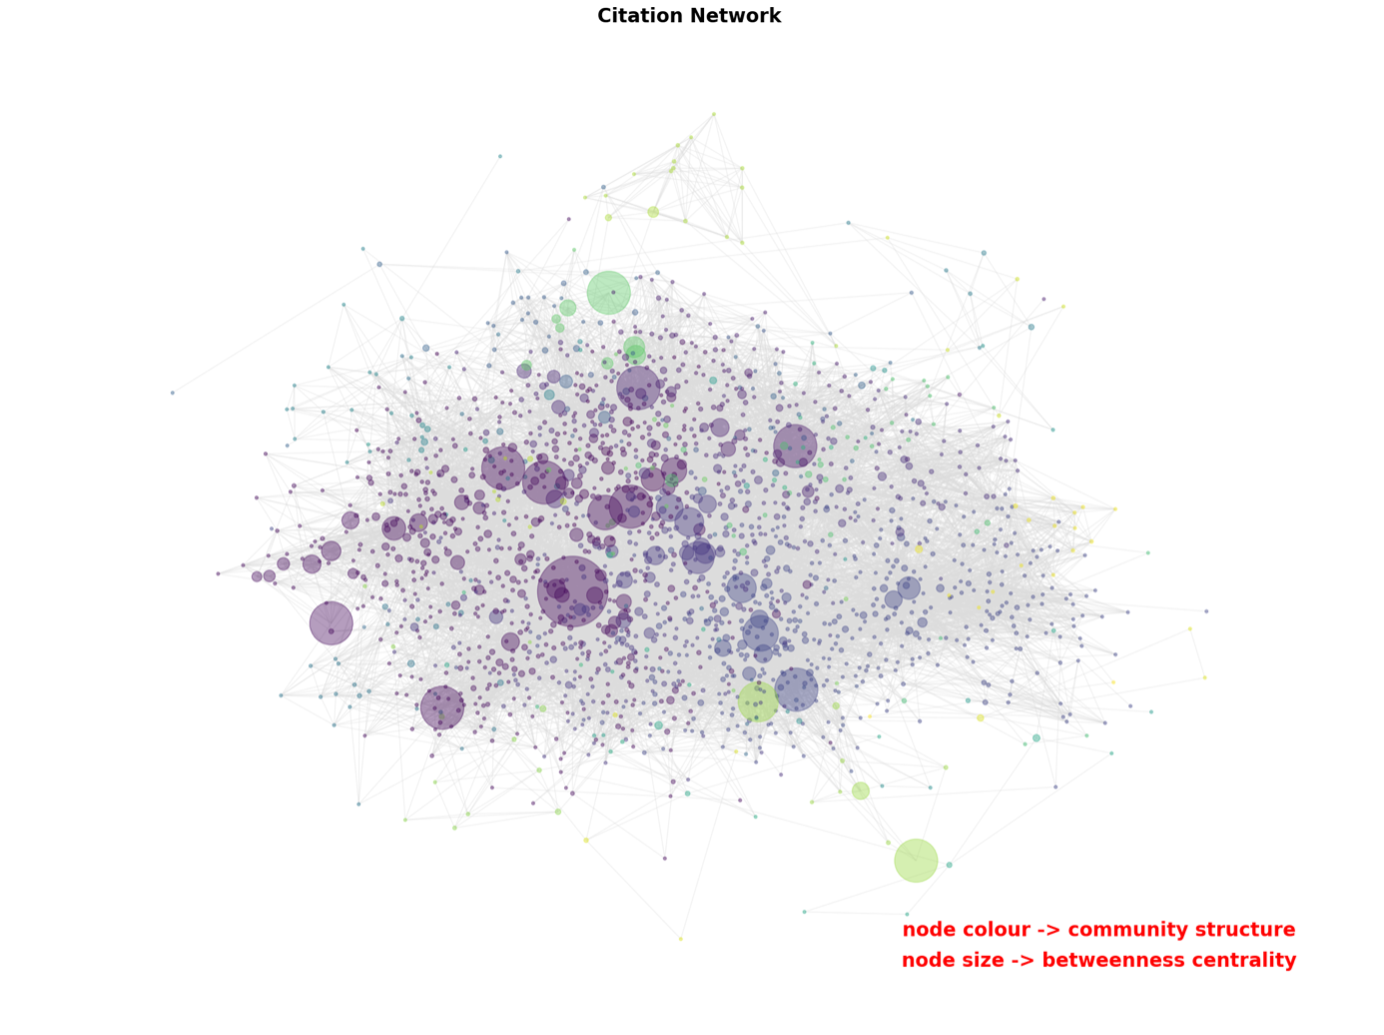
\includegraphics[width=\textwidth]{Figures/Betweenness Centrality.png}
    \caption{Complete citation network}
    \label{fig:network_graph}
\end{subfigure}
\hfill
\begin{subfigure}[b]{0.48\textwidth}
    \centering
    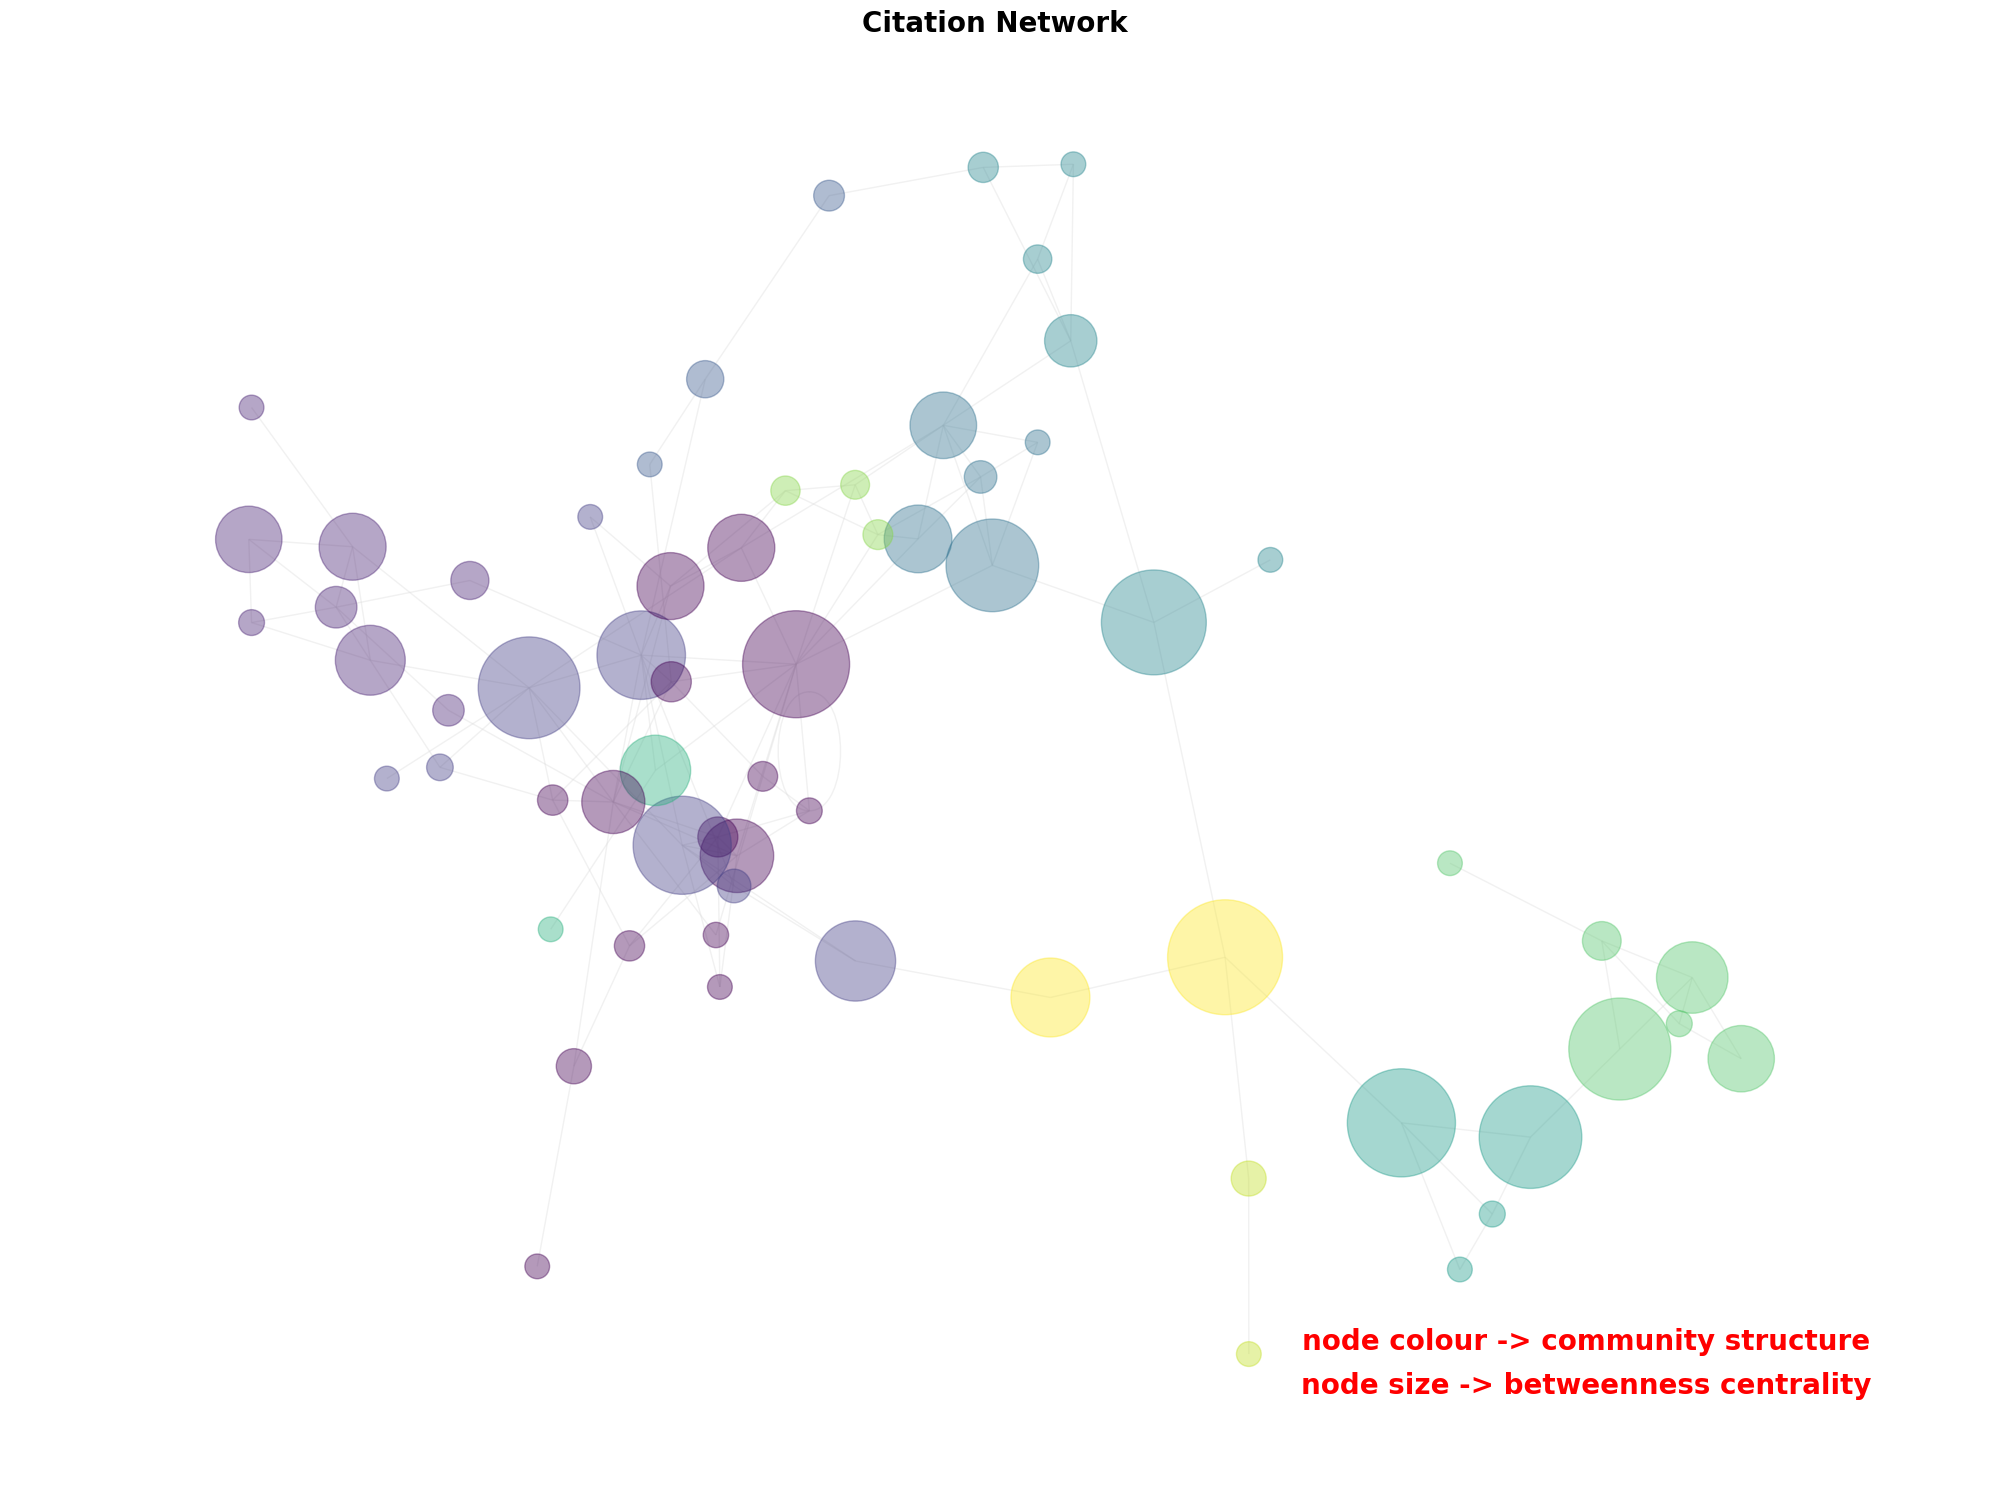
\includegraphics[width=\textwidth]{Figures/Sample Betweenness.png}
    \caption{Sample nodes from the network}
    \label{fig:sample_network}
\end{subfigure}
\caption{Betweenness centrality network graph, same sample nodes from Figure 1 are used here}
\label{fig:combined}
\end{figure}

The above figure visually represents betweenness centrality, where larger nodes indicate higher centrality, and colors represent different communities. In this dataset, theoretical-based and mathematical-based research may form two distinct communities.  

From the figure, it is evident that some nodes act as critical bridges connecting these communities, facilitating the transfer of knowledge between them. The clustering of nodes suggests a dense interconnection within each community, while the sparse links between communities highlight the importance of bridging nodes in uniting separate fields. These bridging nodes likely play a pivotal role in advancing interdisciplinary research.

\subsubsection{In-degree Centrality}
This centrality is straightforward, suggesting that more citations (in-degree to the node) indicate stronger academic importance of the paper (node). This is a standard definition of centrality, modified to ignore the outdegree of a node. The reason for this modification is that we are only concerned with how many papers cite a given paper, not how many papers it cites.
 
\[
\text{Centrality} = \frac{k_{\text{in}}}{N - 1}
\]
where \(N\) is the total number of nodes in the network.

\begin{figure}[h]
\centering
\begin{minipage}[b]{0.48\textwidth}
    \centering
    \begin{tabular}{|c|c|}
        \hline
        \textbf{Node ID} & \textbf{Centrality} \\
        \hline
        9711200 & 0.0869 \\
        9802150 & 0.0639 \\
        9802109 & 0.0591 \\
        9407087 & 0.0468 \\
        9610043 & 0.0432 \\
        9510017 & 0.0416 \\
        9908142 & 0.0412 \\
        9503124 & 0.0401 \\
        9906064 & 0.0372 \\
        9408099 & 0.0362 \\
        \hline
    \end{tabular}
    \captionof{table}{Top 10 Nodes by Indegree Centrality}
    \label{tab:top_nodes_by_centrality}
\end{minipage}
\hfill
\begin{minipage}[b]{0.45\textwidth}
    \centering
    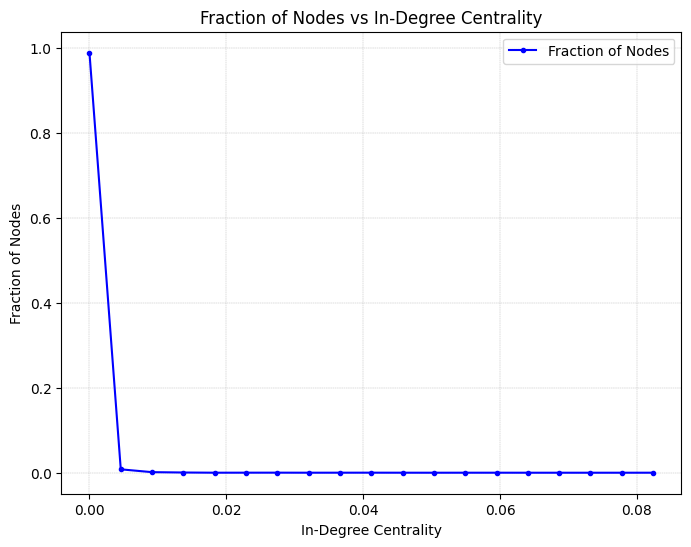
\includegraphics[width=\textwidth]{Figures/Fraction of Nodes Indegree Centrality.png}
    \caption{Fraction of Nodes vs Centrality}
    \label{fig:fraction_vs_centrality}
\end{minipage}
\end{figure}

Figure 6 above shows that majority of the nodes have very low in-degree centrality, indicating that most papers receive few or no citations. The difference in centrality among the top 10 nodes is significantly large, despite there being approximately 27,700 nodes in total. This highlights that only a small fraction of papers have a substantial academic impact, receiving the majority of citations.

In the context of a citation network, this behavior aligns with the power-law distribution often observed in academic citations, where a few highly influential papers dominate the citation landscape. These highly cited papers serve as key resources or foundational works that drive the development and evolution of their respective fields.

\subsection{Cascading Effects}
 In a network, the activity of each node often depends on the activity of its neighboring nodes. Consequently, the failure or inactivity of one node can trigger a chain reaction, causing neighboring nodes to fail or lose significance. In the context of a citation network, if a highly cited paper (a node with high Indegree centrality) becomes inaccessible or discredited, it can disrupt the research built upon it. Subsequent works relying on this paper may lose credibility, leading to a broader impact on the academic community and potential fragmentation of the network.  

To analyze this phenomenon, I build a model where I systematically remove a key node and observe the impact on the network structure. This helps to understand how the removal of influential nodes affects connectivity, community structure, and overall network robustness.

\subsubsection{Model}
Let \( G = (V, E) \) be a directed graph where \( V \) is the set of nodes (researchers) and \( E \) is the set of directed edges (citations). Initially, we remove a node \( v_r \in V \).

\[
N_{out}(v_r) = \{ v_i \mid (v_r, v_i) \in E \}
\]
Let \( R_t \) represent the set of nodes removed at time \( t \). For each removed node \( v_j \), remove all nodes \( v_i \) such that \( (v_j, v_i) \in E \). This chain reaction continues:
\[
R_{t+1} = R_t \cup \bigcup_{v_i \in R_t} N_{out}(v_i)
\]

After the chain reaction ends, the fraction of remaining nodes is:
\[
f_{\text{remaining}} = \frac{|V| - |R_{\text{final}}|}{|V|}
\]

\subsubsection{Impact of Key Nodes }
In this part, the goal is to analyze the fraction of nodes remaining after iteratively removing nodes with the highest in-degree centrality and observing the cascading effects.

The node \( v_r \in V \) with the highest In-degree centrality is removed first:

\[
C_{\text{in}}(v) = \deg_{\text{in}}(v) = \left| \{ u \mid (u, v) \in E \} \right|
\]

Remove \( v_r \) where \( C_{\text{in}}(v_r) \) is maximum.

\begin{figure}[h]
\begin{center}
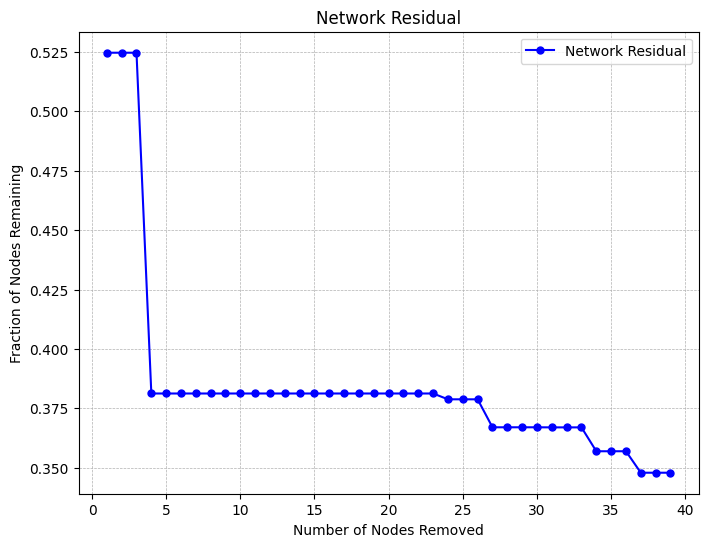
\includegraphics[width=0.7\textwidth]{Figures/Network Residual.png}
\end{center}
\caption{Network residual Vs No of Nodes with high centrality removed}
\end{figure}

Figure 7 below plots the fraction of nodes remaining versus the number of nodes removed. A sharp drop occurs after removing the 4th node (Node ID9407087)\footnote{Title: *Monopole Condensation, And Confinement In N=2 Supersymmetric Yang-Mills Theory*. Authors: N. Seiberg and E. Witten. Published: July 15, 1994.}.
, suggesting its important role in the citation network.

1.	The removal of the 4th node (Node ID:9407087) caused the network size to drop by half, suggesting its critical role in the network.\\
2.	Subsequent high-centrality nodes also caused drops in network size, but the magnitude of these drops diminished, reflecting their reduced structural significance.\\
3.	Innovative papers like (Node ID:9407087) contribute uniquely to the network, causing greater fragmentation compared to highly cited papers conducting similar research.\\
4.	The effect of node removal highlights the dependency of certain high-centrality nodes on others, as their influence is limited when the most critical nodes are removed.


\subsection{Temporal Analysis}
Temporal analysis studies how a network evolves over time, focusing on changes in its structure and the roles of its nodes. In citation networks, this is especially important as academic works accumulate citations over the years, which can alter their significance and influence within the network. Temporal patterns provide insights into research trends, shifts in academic focus, and the emergence of influential works. Here, I specifically analyze the trends in the growth of nodes and edges in the network and the variation in the average in-degree (citations per node) over time.

\begin{figure}[h]
\centering
\begin{subfigure}[b]{0.48\textwidth}
    \centering
    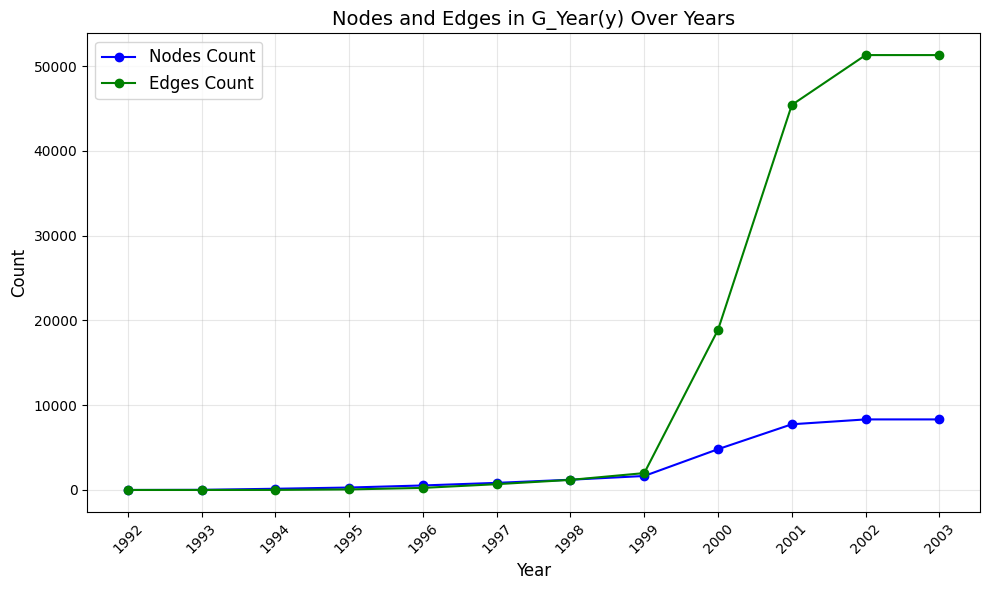
\includegraphics[width=\textwidth]{Figures/Trend change.png}
    \caption{Total Nodes/Edges Vs Year}
    \label{fig:network_graph}
\end{subfigure}
\hfill
\begin{subfigure}[b]{0.48\textwidth}
    \centering
    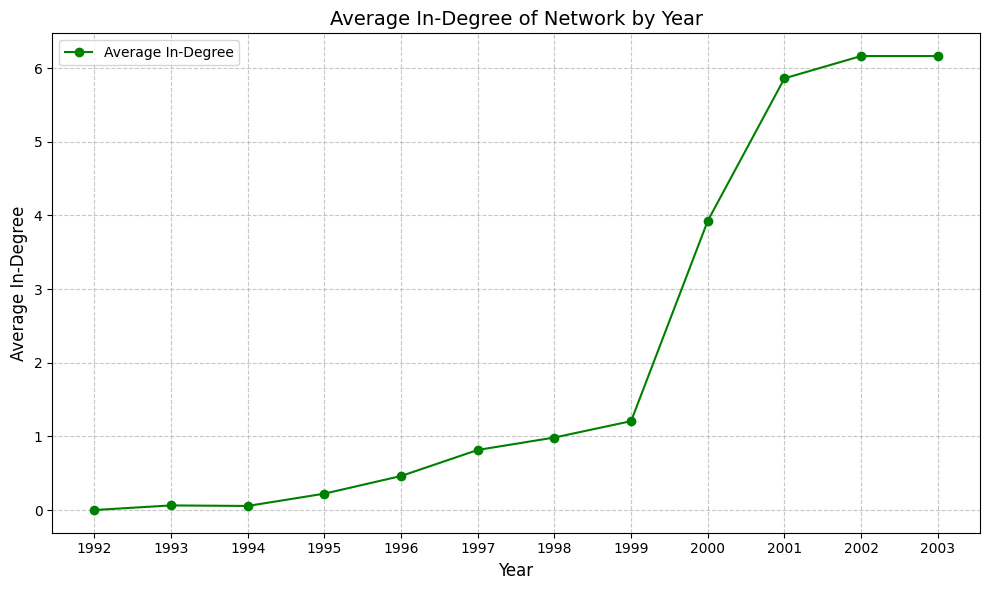
\includegraphics[width=\textwidth]{Figures/CItation Aging.png}
    \caption{Average Indegree Vs Year}
    \label{fig:sample_network}
\end{subfigure}
\caption{Evolution trends of the citation network from 1992 to 2003}
\label{fig:combined}
\end{figure}

Figure 8(a) shows that the number of edges increases more rapidly than the number of nodes. This trend is expected, as the addition of a single node typically introduces at least one edge. However, the rapid rise in edges indicates frequent citations of existing works, which could suggest a consolidation of knowledge rather than the introduction of entirely novel ideas. This pattern also highlights that papers are becoming increasingly interconnected. The disproportionate growth in edges might reflect evolving referencing practices or the availability of more comprehensive databases, making it easier for researchers to locate and cite prior works. This phenomenon also aligns with the idea of cumulative advantage, where older papers gain a significant share of total citations over time.

Figure 8(b) shows that the average in-degree of the network rises consistently but with a slower rate of increase after 1999. This suggests that while older papers accumulate citations, their relative impact diminishes as the network grows, also known as citation aging. A noticeable spike after 1999 may point to improved citation practices, stricter academic standards, or a surge in impactful research. However, more observations would be required from subsequent years to confirm this. The flattening slope in the average in-degree could indicate saturation in the citation process, where foundational works are already well-established, and newer papers struggle to achieve similar levels of influence.

\section{Discussion}
\label{headings}
The analysis confirms that the citation network is scale-free, as evidenced by its degree distribution. A small fraction of papers dominate citations, reinforcing the theory of cumulative advantage. The degree correlation indicates knowledge clusters but limited diversity in connections. Centrality metrics reveal a few critical nodes—acting as bridges between communities or hubs of knowledge—play a disproportionate role in the network’s structure.

The cascading model highlights the fragility introduced by key nodes, such as Node ID: 9407087, whose removal halved the network size. This shows the impact of innovative papers compared to highly cited but interconnected ones. Temporal analysis shows a rapid increase in edges relative to nodes, reflecting growing inter-connectivity and evolving referencing practices. The phenomenon of citation aging is evident, with older papers accumulating citations at a diminishing rate.

Future work could explore the temporal dynamics of citation networks in greater depth by integrating abstract data and linking shifts observed in the model to established academic impact measures, such as the h-index. This approach would involve analysing how structural changes in the network, such as the change in the centrality of specific nodes, correlate with the academic influence of the papers they represent. For instance, papers with high centrality or significant cascading effects might also exhibit high h-indices or other impact metrics. Additionally, studying how emerging papers integrate into or disrupt citation clusters may reveal trends in interdisciplinary research or shifts in focus over time, highlighting periods of increased citation activity tied to breakthroughs or evolving methodologies.


\section{Conclusion}
\label{headings}

In this project, I applied network theory to analyze empirical citation data, focusing on key aspects such as degree distribution, centrality measures, cascading effects, and temporal dynamics. The findings confirm that citation networks are scale-free, with a small fraction of highly influential papers dominating the network. The cascading model further emphasize the importance of innovative, less interconnected works. Temporal trends reveal increasing inter connectivity, evolving citation practices and also highlights the phenomenon of citation aging, where older works accumulate citations at a diminishing rate as newer research emerges.

This study contributes to understanding how citation networks evolve and function as a representation of academic influence. Future research could build on these insights by linking structural metrics with established measures like the h-index to assess academic strength, and by exploring how emerging research integrates into or disrupts existing citation clusters. Such analyses could provide valuable perspectives on academic trends, the dynamics of interdisciplinary collaboration, and the long-term impact of innovative works.

\subsubsection*{Acknowledgments}

I want to thank Prof. Abhishek Samantray for offering the course HSN 619 and giving me this project opportunity. Working on this project has been a great learning experience for me. I’ve gained a lot of knowledge, especially in using LaTeX and improving my documentation skills, which I really enjoyed learning along the way.

The process of exploring network theory concepts and applying them to real empirical data was fascinating and gave me a deeper appreciation for the subject. I truly enjoyed reading Barabási’ book and diving into concepts while working through this project.

\subsubsection*{References}
\small{
[1] \url{https://snap.stanford.edu/class/cs224w-2017/projects/cs224w-68-final.pdf}.

[2] Barabási, A.-L. (2016). {\it Network Science}. Cambridge University Press. Available online at \url{http://networksciencebook.com/}.

[3] Hagberg, A. A., Swart, P. J., \& Schult, D. A. (2008). NetworkX. Software available at \url{https://networkx.org}.
{\bf 15}(7):5249-5262.

[4] Lehmann, S., Lautrup, B., \& Jackson, A. D. (2003). Citation networks in high energy physics. {\it Physical Review E}, {\bf 68}(2): 026113. \url{https://doi.org/10.1103/PhysRevE.68.026113}.

[5] Leskovec, J. \& Krevl, A. (2014). SNAP Datasets: Stanford Large Network Dataset Collection. Retrieved from \url{http://snap.stanford.edu/data}.

}

\end{document}
